% % include the figures path relative to the master file
% \graphicspath{ {./content/results/figures/} }

\section{Experiments and Validation}\label{sec:exp}


To evaluate the effects and influence of different stages of our framework, we perform various tests using our own dataset and sake of comparison, the optimal configurations are evaluated on a public dataset. A detailed description of both datasets can be found in \Cref{sec:exp:dataset}.
For all the experiments, \ac{lbp} and \ac{lbptop} features are extracted for different sampling points of 8, 16, and 24 for radius of 1, 2, and 3, respectively.
As previously mentioned, two different mapping strategies, \emph{local} and \emph{global}, are used.

\added[id=moj]{
In this research we consider a ($7 \times 7$) \acf{sw} for 2D \ac{lbp} and ($ 7 \times 7 \times 7$)  sub-volume for \ac{lbptop}.}
%\emph{Global} mapping considers to extract the features from the 2D B-scans for \ac{lbp} and 3D volume for \ac{lbptop}. 
%Therefore for a volume with $d$ B-scans, the \emph{global}-\ac{lbp} feature leads to a final descriptor of size $d \times \ac{lbp}_{hist}$ and \emph{global}-\ac{lbptop} feature returns the final descriptor of size $3 \times \ac{lbp}_{hist}$.
%Here $\ac{lbp}_{hist}$ refers to the size of uniform and rotation invariant \ac{lbp} histogram which it's number of bins depends on the number of sampling points in a given neighborhood. 
%
%In \emph{local} mapping, the features are extracted from a set of 2D patches for \ac{lbp} and a set of sub-volumes for \ac{lbptop}.
%In this research we consider a ($7 \times 7$) \acf{sw} for 2D \ac{lbp} and ($ 7 \times 7 \times 7$)  sub-volume for \ac{lbptop}. 
%Using these elements, the \emph{local}-\ac{lbp} approach provides a final descriptor of size ($d \times N \times \ac{lbp}_{hist}$) while \emph{local}-\ac{lbptop} results in a final descriptor of size $\frac{d}{7} \times N \times 3 \times \ac{lbp}_{hist}$.
%Here $N$ is the total number of elements in each B-scan, and 3D volume, respectively.

The \emph{global} and \emph{local} extracted features are then presented in low or high representation.
As previously mentioned, \ac{bow} approach is used for high-level representation.
In this regard, to find the optimal number of ``visual-words'' ($k$), we perform a preliminary experiment. 

Using \ac{bow} approach to find the optimal number of ``visual-words'' ($k$), we perform a preliminary classification where different number of words randomly are selected.
In this setup, the words are randomly selected using $k$-means++ algorithm~\cite{arthur2007k}.
This test is performed for all the high-level feature sets considering different pre-processing steps.
The obtained results of this test is represented in experiment~\#1.
Beside this experiment, four other experiments are performed which are explained in the following.
For the sake of comparison all the experiment are performed using all the aforementioned classifiers.
However only the relevant part and results related to our experiment is represented within the paper, while the rest are mentioned in the appendix.

The pipeline in each experiment is evaluated using \ac{lopocv} strategy.
In this validation, at each round a pair \ac{dme}-normal volume is selected for testing while the rest of the volumes are used for training.
The use of this method implies that no variance in terms of \ac{se} and \ac{sp} can be reported.
However, and despite this limitation, \ac{lopocv} has been employed due to the small size of the dataset.

The obtained results of all the experiments except experiment \#1 is represented in terms of \ac{se} and \ac{sp}.
These statistics are driven from the confusion matrix (see Fig.~\ref{fig:CM}).

\begin{figure}
\begin{center}
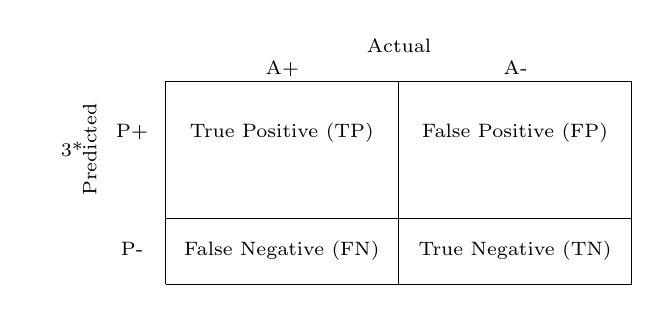
\begin{tikzpicture}[scale=0.4]
      \node at (1,1){
      \scriptsize{
        \begin{tabular}{
            >{\centering}m{1em} >{\centering}m{1em} >{\centering}m{1in} >{\centering\arraybackslash}m{1in}}
          % c>{\centering}m{2em}ccc}
          & & \multicolumn{2}{c}{ Actual}\\
          & & A+ & A- \\
          \cline{3-4}
          & \multicolumn{1}{c|}{} & \multicolumn{1}{c|}{} & \multicolumn{1}{c|}{}\\
          \multirow{3}{*}{\rotatebox[origin=c]{90}{Predicted}}& \multicolumn{1}{c|}{P+} &  \multicolumn{1}{c|}{True Positive (TP)} & \multicolumn{1}{c|}{False Positive (FP)} \\
          &\multicolumn{1}{c|}{}  & \multicolumn{1}{c|}{}& \multicolumn{1}{c|}{} \\
          \cline{3-4}
          & \multicolumn{1}{c|}{} &\multicolumn{1}{c|}{} & \multicolumn{1}{c|}{}\\
          
          & \multicolumn{1}{c|}{P-} &\multicolumn{1}{c|}{False Negative (FN)}  &\multicolumn{1}{c|}{True Negative (TN)}\\
          & \multicolumn{1}{c|}{} &\multicolumn{1}{c|}{} & \multicolumn{1}{c|}{}\\
          \cline{3-4}
          \end{tabular}
      }};
    \end{tikzpicture}
    \end{center}
\caption{Confusion matrix with truly and falsely positive detected samples (\acs{tp}, \acs{fp}) in the first row, from left to right and the falsely and truly negative detected samples (\acs{fn}, \acs{tn}) in the second row, from left to right.}
\label{fig:CM}
\end{figure}
The former evaluate the performance of the classifier with respect to the positive class, while the later evaluate it's performance with respect to negative class.
These measurements are formulated as: 
\begin{align}
 \ac{se}  = \frac{TP}{TP+FN} \qquad \ac{sp} = \frac{TN}{TN+FP}
\end{align}

In experiment \#1 we use \ac{acc} and \ac{f1} instead.
\acl{acc} is used to have a overall sense of classifier performance, and \ac{f1} is used to see the trade off between \ac{se} and precision.
Equation.~\ref{eq:accf1} shows the formulation of these measurements. 
\begin{align}
\ac{acc} = \frac{TP+TN}{TP+TN+FP+FN} \qquad \ac{f1} = \frac{2TP}{2TP +FP+FN}
\label{eq:accf1}
\end{align}


\subsection{Datasets}\label{sec:exp:datasets}

The majority of the development of our framework has been carried out using our own dataset (SERI) and to facilitate further comparison we use the Duke public dataset to evaluate our optimal configurations.

\begin{description}

\item[SERI]- datasets were acquired by Singapore Eye Research Institute (SERI), using CIRRUS TM (Carl Zeiss Meditec, Inc., Dublin, CA) \ac{sdoct} device. The datasets consist of 32 \ac{oct} volumes (16 \ac{dme} and 16 normal cases). Each volume contains 128 B-sane with  dimension of 512 $\times$ 1024 pixels.  All \ac{sdoct} images are read and assessed by trained graders and identifies as normal or \ac{dme} cases based on evaluation of retinal thickening, hard exudates, intraretinal cystoid space formation and subretinal fluid.

\item[Duke] - datasets published by Srinivasan et al. \cite{Srinivasan2014} were acquired in Institutional Review Board-approved protocols using Spectralis \ac{sdoct} (Heidelberg Engineering Inc., Heidelberg, Germany) imaging at Duke University, Harvard University and the University of Michigan. This datasets consist of 45 \ac{oct} volumes (15 \ac{amd}, 15 \ac{dme} and 15 normal). In this study we only consider a subset of the original data containing 15 \ac{dme} and 15 normal \ac{oct} volumes.

\end{description}


% \subsection{Experiments \& Results}
% The performed experiments are listed in the following:\\
%%Both datasets are filtered to attenuate the effect of speckle noise.
%%SIRE dataset is processed using \ac{nlm} as stated in Sect.\,\ref{subsec:prepro}.
%%The different parameters were empirically tested and fixed such that the patch size, the search window and the filtering parameter were set to $(15 \times 15)$, $(35 \times 35)$ and $0.4$, respectively.
%%However, Duke dataset is already filtered using BM3D method~\cite{Srinivasan2014}.
%%For both datasets, \ac{lbp} and \ac{lbptop} features are extracted for different sampling points of 8, 16 and 24 for radius of 1, 2 and 3, respectively.
%%Two different mapping strategies are used: (i) \emph{global} mapping corresponding to the 2D B-scan for \ac{lbp} or the 3D volume for \ac{lbptop} and (ii) \emph{local} mapping considering to a set of 2D \ac{sw} of size $(7 \times 7)$ for \ac{lbp} or the 3D sub-volume for \ac{lbptop} of size $(7 \times 7 \times 7)$.


\subsection{Experiment \#1}
This experiment, conducted on SERI dataset, is performed to find the optimal number of words for \ac{bow} high-level feature representation.
\emph{Global} and \emph{local}-\ac{lbp} and \emph{local}-\ac{lbptop} feature descriptors are re-represented using \ac{bow} approach.
In this experiment, the \ac{bow} algorithm is performed using various number of words in the range of $\{10, 20, 30, \cdots,$
 $100, 200, \cdots, 500, 1000\}$.
The words are randomly selected using $k$-means++ algorithm and the features are mapped to their nearest word to create the final clusters.
In this experiment in order to asses the effect of number of words, simple linear classifier such as \ac{lr} is used.
The number of words associated with highest \ac{acc} and \ac{f1} score, is selected as the optimum number of words.
Table~\ref{tab:Table1} shows the obtained results of this experiment.
The optimum number of words and the achieved \ac{acc} and \ac{f1} of \ac{lr} classifier for different configurations are listed in this table.


  \begin{table}[h]
\caption{ Experiment \#1 - Obtained results of classification using SERI and Duke datasets.}% using \ac{rf} with 100 trees. High-level features with \ac{bow} are obtained with $K$ = 32 visual-words.}
\centering
\resizebox{1\linewidth}{!}{

\begin{tabular}{l lr c lr c lr  c  lr c lr c lr}
\toprule
Features & \multicolumn{8}{c}{SERI dataset} & & \multicolumn{8}{c}{Duke dataset}\\
\cmidrule(l){2-9} \cmidrule(l){11-18}
 	& \multicolumn{2}{c}{$\{8,1\}$}& & \multicolumn{2}{c}{$\{16,2\}$}& &\multicolumn{2}{c}{$\{24,3\}$} & & \multicolumn{2}{c}{$\{8,1\}$}& & \multicolumn{2}{c}{$\{16,2\}$}& &\multicolumn{2}{c}{$\{24,3\}$}\\
  \cmidrule(l){2-3}  \cmidrule(l){5-6}  \cmidrule(l){8-9} \cmidrule(l){11-12}  \cmidrule(l){14-15}  \cmidrule(l){17-18}
	       & \ac{se} & \ac{sp} & & \ac{se} & \ac{sp} & &  \ac{se} & \ac{sp} & &  \ac{se} & \ac{sp} & &  \ac{se} & \ac{sp} & &  \ac{se} & \ac{sp} \\
\midrule
  	%\ac{lbp}					& 43.7 & 43.7 & & 37.5 & 50.0 & & 50.00 & 62.50  \\
 	\emph{global}-\ac{lbptop}				       & 56.2 & 62.5 & & \textbf{87.5} & \textbf{75.0} & & 68.7 & 68.7 & & 80.0 & 93.3 & & 73.3 & 86.6 & & 73.3 & 86.6 \\
	%\ac{lbp}+\ac{bow}		& 50.0 & 81.2 & & 57.5 & 68.7 & & 50.0 & 50.0 \\
	\emph{local}-\ac{lbp}	   & \textbf{75.0} & \textbf{87.5} & & 81.2 & 75.0 & & 68.7 & 62.5 & & \textbf{80.0} & \textbf{86.6} & & \textbf{86.7} & \textbf{100} & & 93.3 & 86.6\\
	\emph{local}-\ac{lbptop}   & 62.5 & 68.7 & & 56.2 & 37.5 & & 37.5 & 43.7 & & 80.0 & 86.6 & & 86.6 & 86.6 & & 60.0 & 80.0 \\
\bottomrule
\end{tabular}}
\label{tab:table1-1}
\end{table}







Figure.~\ref{fig:RBOW} shows the obtained graphs for some of the configurations. \\




 
\subsection{Experiment \#2}
\deleted[id=sik]{Experiment \#2} is performed for high-level features on SERI dataset as well. 
In this experiment using the optimum number of words which are obtained from the previous experiment, the low-level feature sets with regards to different pre-processing configurations are re-represented using \ac{bow} and $k$-means clustering approach and are classified using $k$-\ac{nn} classifier.
\added[id=moj]{$k$-\ac{nn} classifier was chosen since it provides a sense of} 
% local and global \ac{lbp} and local \ac{lbptop}
Table~\ref{tab:table2} shows the obtained results from this experiment.\\


\subsection{Experiment \#3}
\deleted[id=sik]{Experiment \#3} is dedicated to compare the performance of different classifiers.
This experiment is also performed on SERI dataset and for high-level features.
The \added[id=moj]{best configurations} of feature set and pre-processing based on the previous experiment is classified with different classifiers such as \ac{rf}, \ac{gb}, \ac{svm}, \ac{lr} and $k$-\ac{nn}.
The obtained results of this experiment is listed in Table.~\ref{tab:tab3}.\\


\subsection{Experiment \#4}
\deleted[id=sik]{Experiment \#4} is conducted for low-level features.
The \emph{global} \ac{lbp} and \ac{lbptop} features are classified using the same classifiers as previous experiments.
The obtained results from this experiment is listed in Table.~\ref{tab:table4}.\\
 
\subsection{Experiment \#5}
\deleted[id=sik]{Experiment \#5} is performed to evaluate the performance of our proposed framework considering different dataset.
In this regards, the best configuration in terms of low-level or high-level representations, number of words and classifiers obtained from the previous experiments are performed on Duke dataset.
A comparison of the obtained results from SERI and Duke datasets are presented in Table.~\ref{tab:table5}.
  

% The SERI datasets are provided in complete \ac{oct} volumes by 512$\times$1024$\times$128 dimensions. Using this datasets, first the three low-level features such as \ac{lbp}, \ac{lbp}+\ac{pca} and \ac{lbptop} are extracted. The rotation invariant uniform ($riu2$) descriptors are calculated with the $P$ number of 8, 16 and 24 for the radius if 1, 2 and 3 respectively. The features are classified using RF with 100 tress. Table \ref{tab:LbPTopVolumeResult} shows the relative results for $8riu2$, $16riu2$, $24riu2$ and their combination $8riu2 + 16riu2 + 24riu2$. The results are presented in terms of \ac{se} and \ac{sp} percentages.

% The second experiment is carried out using high-level features and \ac{bow} approach, on SERI datasets. The first high-level feature \ac{lbp}+\ac{bow} is obtained by applying \ac{bow} with 32 visual-words on the previously low-level \ac{lbp} features (applied on each B-scan). The second and third high-level descriptors are obtained using a dense approach by applying the \ac{sw} of size (7$\times$7) on each B-scan and \ac{sw} of size (7$\times$7$\times$7) to the whole volume respectively. \ac{lbp}+\ac{bow}+\ac{sw} represent the second high-level feature where the 2D-\ac{lbp} features are extracted for each sliding window on each B-scan and the visual-words are selected from the pool, consisting of their histograms. The third high-level feature, \ac{lbptop}+\ac{bow}+\ac{sw}, is defined using \ac{lbptop}. By using the sliding window the 3D-\ac{lbp} features are extracted for each patch. Same as previous experiment with low-level features, the descriptors are calculated with the $P$ number of 8, 16 and 24 for the radius if 1, 2 and 3 respectively. The obtained results of this experiment are illustrated in Tab. \ref{tab:SERIBoWResult}.

% In order to compare our proposed framework the third experiment is carried out using the subsection of Duke datasets \cite{Srinivasan2014}. The OCT volumes provided by this datasets are of different volume size, cropped and denoised by the method of authors choice. Subsequently only the second experiment with high-level features and low-level \ac{lbptop} features comply with these requirements. The number of visual-words and the size of \ac{sw} for 2D and 3D features are the same than the previous experiment. The 2D and 3D \ac{lbp} features are extracted with $P$ number of 8, 16 and 24 for the radius if 1, 2 and 3 respectively. The obtained results for this experiment are shown in Tab. \ref{tab:DukeBoWResult}.
%----------

%%% Local Variables:
%%% mode: latex
%%% TeX-master: "../../main.tex"
%%% End:
